%% USEFUL LINKS:
%% -------------
%%
%% - UiO LaTeX guides:          https://www.mn.uio.no/ifi/tjenester/it/hjelp/latex/
%% - Mathematics:               https://en.wikibooks.org/wiki/LaTeX/Mathematics
%% - Physics:                   https://ctan.uib.no/macros/latex/contrib/physics/physics.pdf
%% - Basics of Tikz:            https://en.wikibooks.org/wiki/LaTeX/PGF/Tikz
%% - All the colors!            https://en.wikibooks.org/wiki/LaTeX/Colors
%% - How to make tables:        https://en.wikibooks.org/wiki/LaTeX/Tables
%% - Code listing styles:       https://en.wikibooks.org/wiki/LaTeX/Source_Code_Listings
%% - \includegraphics           https://en.wikibooks.org/wiki/LaTeX/Importing_Graphics
%% - Learn more about figures:  https://en.wikibooks.org/wiki/LaTeX/Floats,_Figures_and_Captions
%% - Automagic bibliography:    https://en.wikibooks.org/wiki/LaTeX/Bibliography_Management  (this one is kinda difficult the first time)
%%
%%                              (This document is of class "revtex4-1", the REVTeX Guide explains how the class works)
%%   REVTeX Guide:              http://www.physics.csbsju.edu/370/papers/Journal_Style_Manuals/auguide4-1.pdf
%%
%% COMPILING THE .pdf FILE IN THE LINUX IN THE TERMINAL
%% ----------------------------------------------------
%%
%% [terminal]$ pdflatex report_example.tex
%%
%% Run the command twice, always.
%%
%% When using references, footnotes, etc. you should run the following chain of commands:
%%
%% [terminal]$ pdflatex report_example.tex
%% [terminal]$ bibtex report_example
%% [terminal]$ pdflatex report_example.tex
%% [terminal]$ pdflatex report_example.tex
%%
%% This series of commands can of course be gathered into a single-line command:
%% [terminal]$ pdflatex report_example.tex && bibtex report_example.aux && pdflatex report_example.tex && pdflatex report_example.tex
%%
%% ----------------------------------------------------


\documentclass[english,notitlepage,reprint,nofootinbib]{revtex4-2}  % defines the basic parameters of the document
% For preview: skriv i terminal: latexmk -pdf -pvc filnavn
% If you want a single-column, remove "reprint"

% Allows special characters (including æøå)
\usepackage[utf8]{inputenc}
% \usepackage[english]{babel}

%% Note that you may need to download some of these packages manually, it depends on your setup.
%% I recommend downloading TeXMaker, because it includes a large library of the most common packages.

\usepackage{physics,amssymb}  % mathematical symbols (physics imports amsmath)
\usepackage{amsmath}
\usepackage{graphicx}         % include graphics such as plots
\usepackage{xcolor}           % set colors
\usepackage{hyperref}         % automagic cross-referencing
\usepackage{listings}         % display code
\usepackage{subfigure}        % imports a lot of cool and useful figure commands
% \usepackage{float}
%\usepackage[section]{placeins}
\usepackage{algorithm}
\usepackage[noend]{algpseudocode}
\usepackage{subfigure}
\usepackage{tikz}
\usetikzlibrary{quantikz}
% defines the color of hyperref objects
% Blending two colors:  blue!80!black  =  80% blue and 20% black
\hypersetup{ % this is just my personal choice, feel free to change things
	colorlinks,
	linkcolor={red!50!black},
	citecolor={blue!50!black},
	urlcolor={blue!80!black}}


% ===========================================


\begin{document}
	
	\title{Simulation of the 2D Ising model with Monte Carlo Markov Chain}  % self-explanatory
	\author{} % self-explanatory
	\date{\today}                             % self-explanatory
	\noaffiliation                            % ignore this, but keep it.
	
	%This is how we create an abstract section.
	\begin{abstract}
	We study the 2D ferromagnetic Ising Model with Monte Carlo Markov chain. We use the Metropolis algorithm to sample the probability distribution of the Ising model.
	As proven in 1944 by Lars Onsager$\colorbox{red}{Citation of his paper?}$, we have a phase transition at the critical temperature $T_c(L=\infty)=2.269 \mathrm{J / k}$. We find a matching numerical 
	critical temperature $T_c(L=\infty) = 2.29 \pm 0.04 \mathrm{J / k}$. To verify that the Metropolis algorithm is working correctly, we used the analytical solution in the case 
	of 2x2 lattice. Additionnaly we look at the distribution of our energy normalized by spin $\epsilon$ for a 20x20 lattice with different temperatures. We find that
	we temperature plays an important role in the shape of our distribution. Since we can only compute theoretical values when we reach equilibrium we used the "Burn-in" 
	method to determine the number of cycle needed to reach equilibrium. For a 20x20 lattice, we determine that around 10000 cycles is enough to reach equilibrium.
	  
	\end{abstract}
	\maketitle	
	
	
	% ===========================================
	\section{Introduction} \label{sec:introduction}
	%
	The Ising model is a statistical mechanics model that describes the ferromagnetism by a system of spins on a lattice. 
	Ferromagnetism is a property of certain materials allowing it to form a permanent magnet for example. One important concept in the Ising model for dimension 
	higher than 1 is phase transition. A phase transition is an extreme change in the physical properties. In our case, the model will go high magnetization to close to 
	0 with increasing temperature. $\colorbox{red}{More detail about Ising model? Other use in science perhaps}$\\
	
	There is no analytical solution for the Ising model in dimensions $>$ 2. However, we can use the Monte Carlo Markov Chain (MCMC) algorithm to simulate our model. 
	MCMC was developed in the 40s by Stanislaw Ulam and Jon Von Neumann $\colorbox{red}{Citation of his paper?}$. The basic idea is to use randomness to solve deterministic problem and as shown great 
	results in many situations $\colorbox{red}{some example?}$ in computational physics. In this
	paper we will apply the Monte Carlo methods to solve the 2D Ising Model and we will use the 
	Metropolis algorithm to sample the distribution. As explained in more details in section
	\ref{sec:theory} we will use the relation between finite lattice and infinite lattice to 
	estimate the critical temperature, $T_c(L=\infty)$ solved analytically by Lars Onsager in 1944. \\
	
	In section \ref{sec:theory}, we will introduce a formal explanation of the Ising Model 
	with the analytical solution for the 2x2 case used as a benchmark for our algorithm. In the
	next section \ref{sec:methods} we will discuss the numerical methods and the algorithms 
	used. Section \ref{sec:results} and section \ref{sec:discussion} respectively presents our
	results from our simulation and an analysis of them. Finally section \ref{sec:conclusion} summarize the main points of this paper.   

	\section{Theory}\label{sec:theory}
	\subsection{2D Ising Model} \label{subsec:Ising}
	The 2D Ising model is a 2 dimensional lattice of equal length and row (L) compose of spins
	$s_i$. So an lattice of size L will wield $\rm LxL=N$ spins. Each spin can take one of the
	following values $\{-1,	1\}$ representing their magnetic dipole. Every spin can interact 
	with their next neighbor meaning that every spin can have up to four interactions. One 
	important detail in physics is what to do with the boundaries. In our case we will consider 
	a periodic boundary condition. This means that we will always consider four interactions
	for each spin. This is the geometrical equivalent of having a lattice in the shape of a 
	torus. We will denote the spin configuration by $\textbf{s}=\{s_1, s_2, ..., s_N\}$. This allows us 
	to write the Hamiltonian 
	
	\begin{equation}
		H(\textbf{s}) = -J \sum_{<kl>} s_ks_l + h \sum_{i=1}^{N} s_i \label{eq:hamilton}
	\end{equation}
	
	Eq. \ref{eq:hamilton} is composed of two terms. The first one is the contribution of every 
	neighbors. $<kl>$ represents the neighboring pairs of k and l. $J$ is the coupling constant 
	and represent the strength of spin interaction. In this paper every results have been 
	produce with $J=1$. The second term is here to account for a potential external magnetic 
	field with $h$ acting as the strength of this magnetic field. We will not consider an 
	external magnetic field in this paper so $h=0$ and eq. \ref{eq:hamilton} becomes
	
	\begin{equation}
		H(\textbf{s}) = -J \sum_{<kl>} s_ks_l \label{eq:Hamiltonian}
	\end{equation}
	
	In statistical mechanics we use probability and observables. In our problem we have two 
	observables the magnetization and the energy respectively 
	
	\begin{align}
		M(\textbf{s}) &= \sum_{i=1} s_i \label{eq:M}\\
		E(\textbf{s}) &= H(\textbf{s}) = -J \sum_{<kl>} s_ks_l \label{eq:E}
	\end{align}

	$M$ is the magnetization summing all spins in the lattice. Since we will study these 
	observable for different lattice size we introduce the normalized by spin magnetization and
	energy 
	
	\begin{align}
		m(\textbf{s}) &= \frac{M(\textbf{s})}{N} \label{eq:m} \\   
		\epsilon(\textbf{s}) &= \frac{E(\textbf{s})}{N}  \label{eq:epsilon}
	\end{align}
>>>>>>> refs/remotes/origin/main

	
	Given a temperature $T$ to determine the probability of being in the configuration
	$\textbf{s}$ we will use the Boltzmann distribution with the partition function $Z$
	
	\begin{align}
		p(\textbf{s},T) &= \frac{1}{Z} e^{-\beta E(\textbf{s})} \label{eq:B_probability} \\
		Z &= \sum_{\text{\textbf{s}}} e^{-\beta E(\textbf{s})} \label{eq:partition_fun}
	\end{align}

	where $\beta = \frac{1}{kT}$, $k$ the Boltzmann constant. the summation for the partition
	function means that we iterate over every possible s\textbf{s}. This numbers scale as $2^N$
	showing with analytical calculation of the partition for big lattice becomes quickly 
	impossible. \\
	
	In statistical mechanics we can only experimentally calculate the averaged values of our 
	observable. Meaning that for a discrete observable $A(X)$ with probability $p(X)$ we have 
	\begin{equation}
		<A> = \sum_{X}A(X)p(X) \label{eq:expectation value}
	\end{equation} 
	
	We can then apply eq. \ref{eq:expectation value} to our observables and we can define two 
	values of interest, $C_v$ and $\chi$. The first one is he heat capacity and $\chi$ is the
	magnetic susceptibility 
	
	\begin{align}
		C_v &= \frac{<E^2> - <E>^2}{NkT^2} \label{eq:heat_capacity} \\
		\chi &= \frac{<M^2> - <|M|>^2}{NKT} \label{eq:susceptibility}
	\end{align}
 	
	\subsection{2x2 analytical solution}\label{subsec:analytical solution}
	
	Since it gets quickly impossible to calculate the probability distribution due to the 
	partition function. We will first solve the 2x2 case where we only have $2^4=16$ possible
	$\textbf{s}$. 
	
	\begin{table}[h!]
	\centering
	\begin{tabular}{|c|c|c|c|}
		\hline
		\# $s_i=1$ & E [J/k] & M[1/J] & degeneracy \\
		\hline
		\hline
		0 & -4 &  -4 &  1  \\
		1 & 0&   -2&   4  \\ 
		2 & 0 & 0&  4  \\
		2 & 4 & 0 &  2 \\
		3 & 0  & 2 & 4 \\
		4 & -4 & 4 & 1 \\
		\hline
	\end{tabular}
	\caption{ Summary of all possible energy E, magnetization M and the degeneracy is the 
	number of spin configuration with the same characteristic} \label{tab:summary2x2}
	\end{table} 
	
	Table \ref{tab:summary2x2} shows all possibility in the 2x2 case and we see that summing all
	of the degeneracy gives us 16 assuring us that we covered every single possibility. Now that
	we have found these values. We can proceed in the calculation of the partition function
	
	\begin{equation}
		Z = 12 + 4\cosh(8\beta) \label{eq:Analytical_partition} 
	\end{equation}	

	
	With Table \ref{tab:summary2x2}, eq. \ref{eq:Analytical_partition} and \ref{eq:expectation value} we obtain the following relations 
	
	\begin{align*} \label{eq:sol}
		<E> &= \frac{-32\sinh(8\beta)}{Z}  \\
		<\epsilon> &= \frac{<E>}{4} = \frac{-8\sinh(8\beta)}{Z} \\
		<E^2> &= \frac{256 \cosh(8\beta)}{Z} \\
		<M> &= \frac{32}{Z} (2 + e^{8\beta}) \\
		<M^2> &= \frac{32}{Z} (1 + e^{8\beta}) \\
		<C_v> &= \frac{<E^2> - <E>^2}{4} \\
		<\chi> &=  \frac{<M^2> - <|M|>^2}{4}
	\end{align*}
	
	
	\subsection{Phase transition}\label{subsec:phase transition}
	One of the most interesting physical property of the 2D Ising model is the phase transition.
	It means that for a certain critical temperature $T_c$ our lattice will suddenly magnetizes. For an infinite size model Lars Onsager found in 1944 the theoretical value of 
	
	\begin{equation}
		T_c(L=\infty)=\frac{2}{log(1 + \sqrt{2})} J/k \approx 2.269 J/k \label{Tc_theo}
	\end{equation}
	
	Another important aspect of phase transition is that different system exhibit similar 
	behavior around the critical temperature. This is known as the critical exponents. For the 
	finite size we have \colorbox{red}{Probably quote Morten (found in project description)}. 
	
	\begin{equation}
		\xi \propto |T - T_c(L=\infty)|^{-\nu} \label{eq:critical exponent}
	\end{equation}
	
	with critical exponent $\nu=1$, $\xi$ is the correlation length and the largest possible 
	value is $\xi=L$, which we associate with the critical temperature of our system. \\
	
	With our finite critical temperature $T_c(L)$  we can estimate numerically the infinite
	critical temperature with the scaling relation 
	
	\begin{equation}
		T_c(L) = aL^{-1} + T_c(L=\infty) \label{eq:scaling relation}
	\end{equation}
	
	a is a constant. This allows us to perform a linear regression to find approximate value 
	of the slope (a) and the intersect point, $T_c(L=\infty)$.
	
	% ===========================================
	
	
	\section{Methods}\label{sec:methods}
	%
	\subsection{MCMC and Metropolis algorithm} \label{subsec:mcmc}
	To compute our model we will use the Monte Carlo Markov Chain (MCMC). This method use 
	statistic to study deterministic problem like the Ising model. We define a probability 
	distribution function and sample states from it. After some iteration or cycle we obtain
	ensemble of average which allows us to get an understanding of a system when analytical 
	solution does not exist. \\
	
	A Markov Chain is a stochastic process where each step possess a probability
	independent of the history. Meaning that the only relevant information needed is the 
	latest step to calculate the probability from transitioning but all previous states are
	not necessary. This takes away a lot of constraint where keeping track of history would
	rise big memory issue. Fortunately this is not the case here. \\
	
	For the Ising model we have define the distribution probability
	
	\begin{equation}
		p_{\rm \textbf{s}} = \frac{e^{-\beta E(\textbf{s})}}{Z} \label{eq:prob distribution}
	\end{equation}	 
	
	
	Now we will need two assumption. The first one is ergodicity. This means that every state
	can be reach within a finite amount of time. This allows us to consider every states possibles
	as we assume that no state can possibly prevent us from reaching equilibrium (the states 
	with the biggest probability). We also use detailed balance. This means that if we have
	two states $P_1$ and $P_2$ we have as much of transition from state 1 to 2 then 2 to 1. Here
	this means that:
	
	\begin{align}
		P_1 T(1:2) &= P_2T(2:1) \\
		\frac{T(1:2)}{T(2:1)} &= \frac{P_2}{P_1} \\ 
		&= e^{-\beta \Delta E} \label{eq:deltaE}
	\end{align}

	where $T(i:j)$ denotes the transition probability of going to state i to j. The last line 
	is obtained when we replace the $P_i$ with eq \ref{eq:prob distribution}. \\
	
	However we do not know what the actual transition probability is but we do not need to know
	it with the Metropolis algorithm. This algorithm creates an acceptance function that respect
	the constraint of our system and is use to represent our transition probability. We assume 
	that our transition probability should be depend of \ref{eq:deltaE}. This gives us
	
	\begin{equation}
		T(1:2) = \text{min}(1, e^{-\beta \Delta E\\}) \label{eq:metropolis}
	\end{equation}
	
	
	This equation satisfies all of our constraints. We can see that the transition can only
	take values between 0 and 1. 
	
	% ===========================================
	\subsection*{The algorithm}\label{subsec:you suck eloi}
	%
	
	We create a lattice of size $L \times L $ full of spin of values \{-1, 1\}. Since we 
	consider boundary conditions we use the modulo operator to access the spin at the beginning
	or end of our lattice once we reach the opposite side while calculating the Hamiltonian. We
	initialize our lattice either randomly or ordered with all spin in the up position (value
	of 1). \\
	
	Once that we have initialize our system with the correct temperature and a random initial
	state. We start the our Monte Carlo algorithm. One cycle correspond of N spin flip attempt. 
	N being the total number of spin. We take one random spin, we flip it, calculate the 
	energy difference and we have three options. If $\Delta E \le 0 $ we accept the state, 
	change our lattice and compute the magnetization and the energy. If $\Delta E > 0$, we have
	two possibility. We will draw a random number u between 0 and 1 from a uniform distribution
	and if $u < \Delta E$ we accept the new state. If that is not the case we refuse the state
	keep our current state and add their energy and magnetization to our data once more. \\
	
	We will compute $K$ number of cycle but we will keep only $K - N_{\rm burn}$ values 
	because in statistical mechanics we need to reach equilibrium to match the experimental. 
	This methods is called the burn-in method and consist in assuming that $N_{\rm burn}$ cycle
	is enough to reach equilibrium in our system. The determination of this value will be 
	discussed in more detail in Section \ref{subsec: burn in estimation}. \\
	
	Finally, to accelerate our computational time we will use parallelization with OpenMP. We 
	will use it when we will run simulation for a lot of temperature while studying the 
	phase transition. This will allow us to parallelize the temperature loop as each iteration
	are independent from each other. This operation reduced our computing time up to $50\%$. 

	% ===========================================
	\section{Results}\label{sec:results}
	%
	\subsection{2x2 numerical simulation}\label{subsec: 2x2 numerical}
	We used $T=1 J/k$ and ran the simulation for \{500, 1000, 2000, 3000, 4000, 5000, 6000, 
	7000, 8000, 9000, 10000, 20000, 30000, 40000, 50000, 60000, 70000, 80000, 90000, 100000\}
	cycles and $L=2$. We computed the analytical solution described in Section \ref{subsec:analytical solution}. 
	Figures \ref{fig:chi4} and \ref{fig:cv4} shows the expected value of $\chi$ and $C_v$ for different number of cycle done. The theoretical values is plotted in dashed line. We did
	not represented $<m>$ or $<E>$ as they are a necessity to compute $\chi$ and $C_v$ so 
	finding good results for the last two shows that we have evaluated correctly the other
	quantities. 
	
	\begin{figure}[h!]
		\centering
		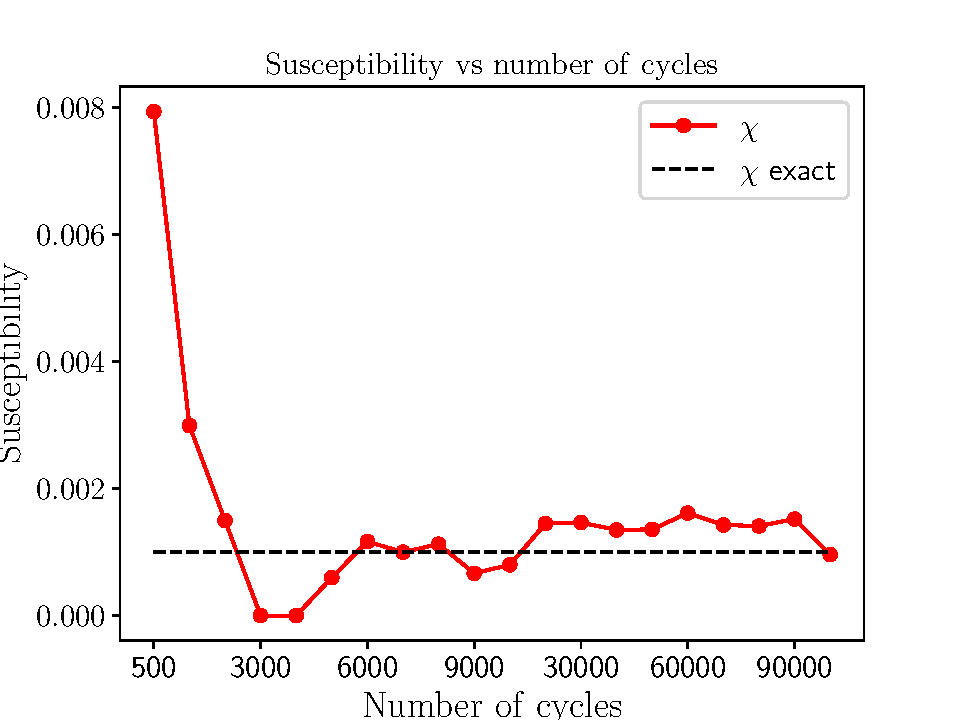
\includegraphics[scale=0.55]{figures/chi_problem4.pdf}
		\caption{}
		\label{fig:chi4}
	\end{figure}

	\begin{figure}[h!]
		\centering
		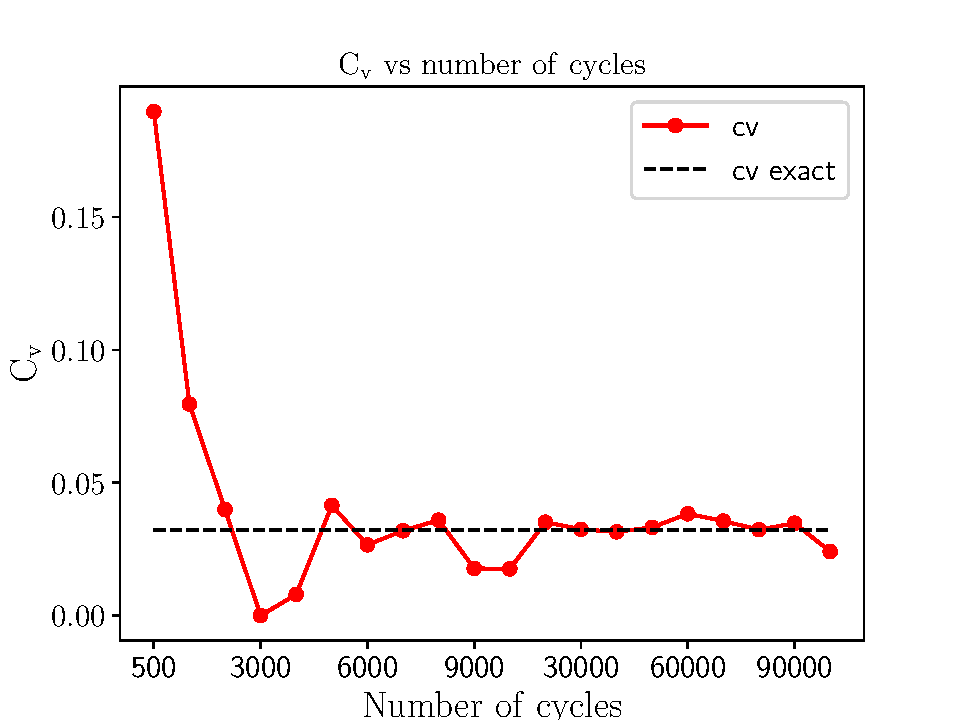
\includegraphics[scale=0.55]{figures/CV_problem4.pdf}
		\caption{}
		\label{fig:cv4}
	\end{figure}
	
	\subsection{Burn-in time estimation}\label{subsec: burn in estimation}
	
	For the Burn-in testing we took the same number of cycle as Section \ref{subsec: 2x2 numerical},
	with $L=20$ instead of $L=4$. We used two different temperatures $T_1=1 J/k$ and $T_2=2.4 J/k$
	starting from ordered (all spin being 1) and random. We plotted the expected value of $m$ 
	and $\epsilon$ according to the number of cycles. The results are presented in 
	Figures \ref{fig:eps5} and \ref{fig:m5}. 
	
	\begin{figure}[h!]
		\centering
		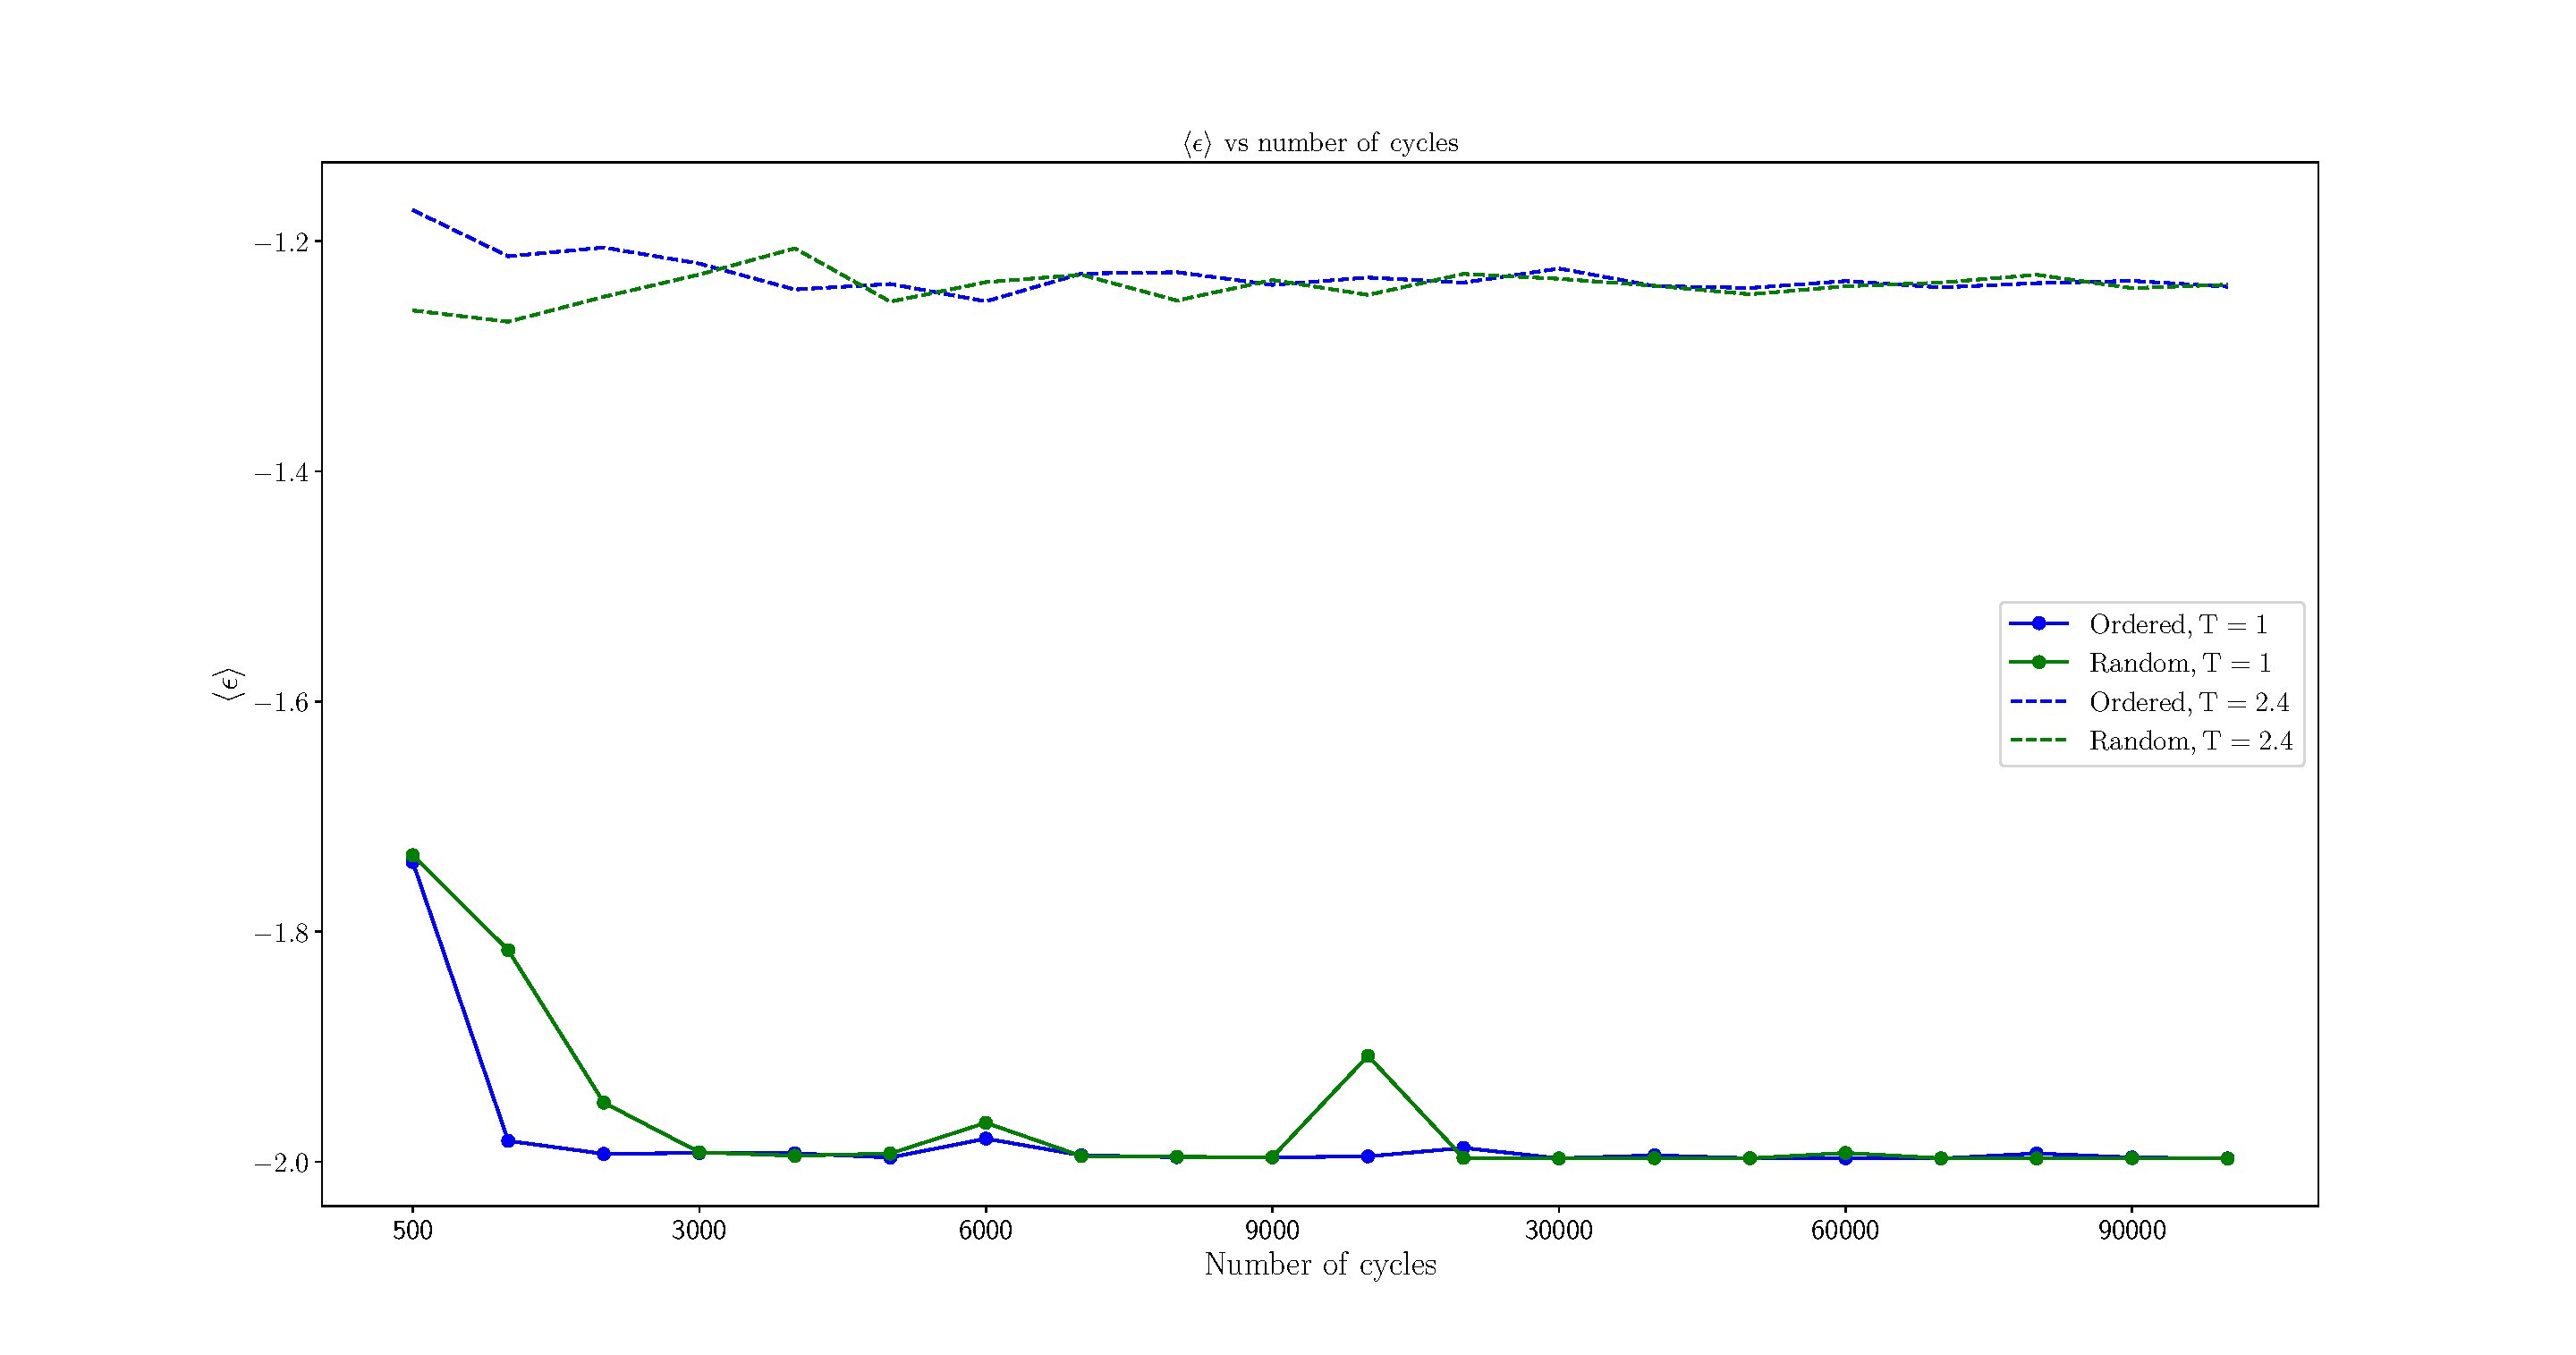
\includegraphics[scale=0.55]{figures/epsilon_problem5.pdf}
		\caption{}
		\label{fig:eps5}
	\end{figure}
	\begin{figure}[h!]
		\centering
		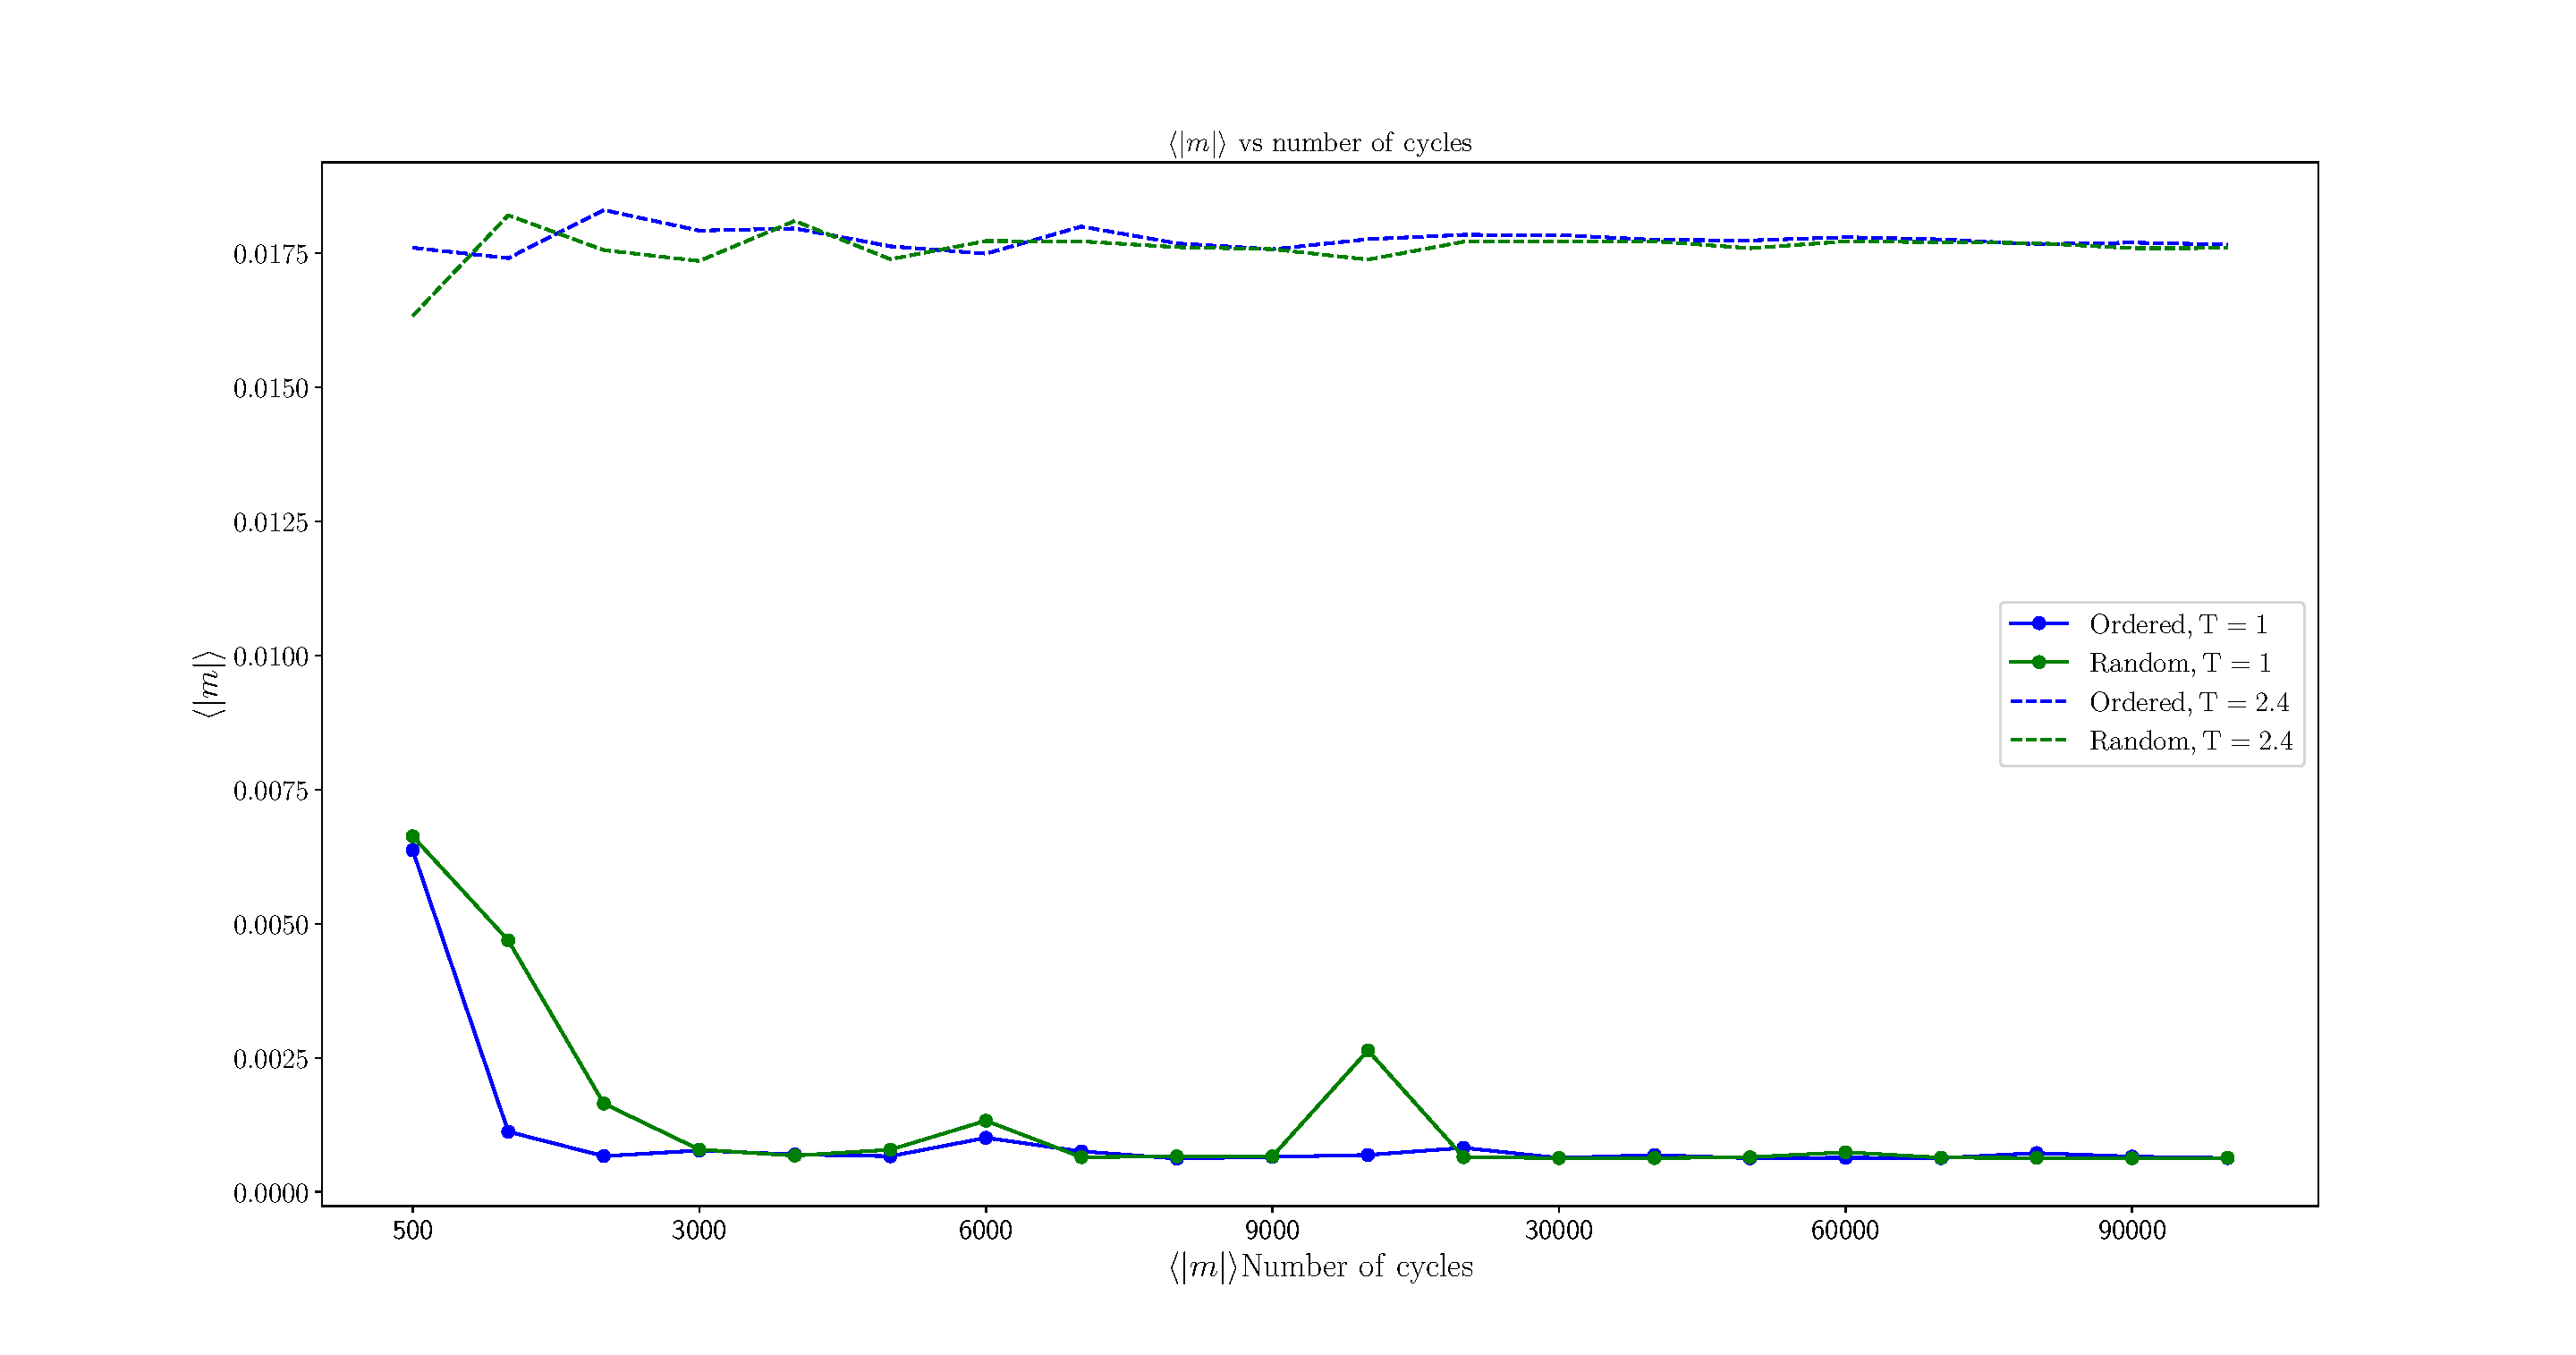
\includegraphics[scale=0.55]{figures/m_problem5}
		\caption{}
		\label{fig:m5}
	\end{figure}

	\subsection{Distribution probability of $\epsilon$}\label{subsec:dist probability}
	
	For the probability distribution of $\epsilon$ we took the data set used in section 
	\ref{subsec: burn in estimation}, so 100000 cycles computed for both temperatures 
	without any burn-in time and starting from random position. Figures \ref{fig:hist1}
	and \ref{fig:hist2} show the histogram of our distribution for their temperature. 
	We also computed the variance and found $\sigma\approx0.00011$ for $T=1 J/k$ and 
	$\sigma\approx0.02023$ for $T=2.4 J/k$.
	
	\begin{figure}[h!]
		\centering
		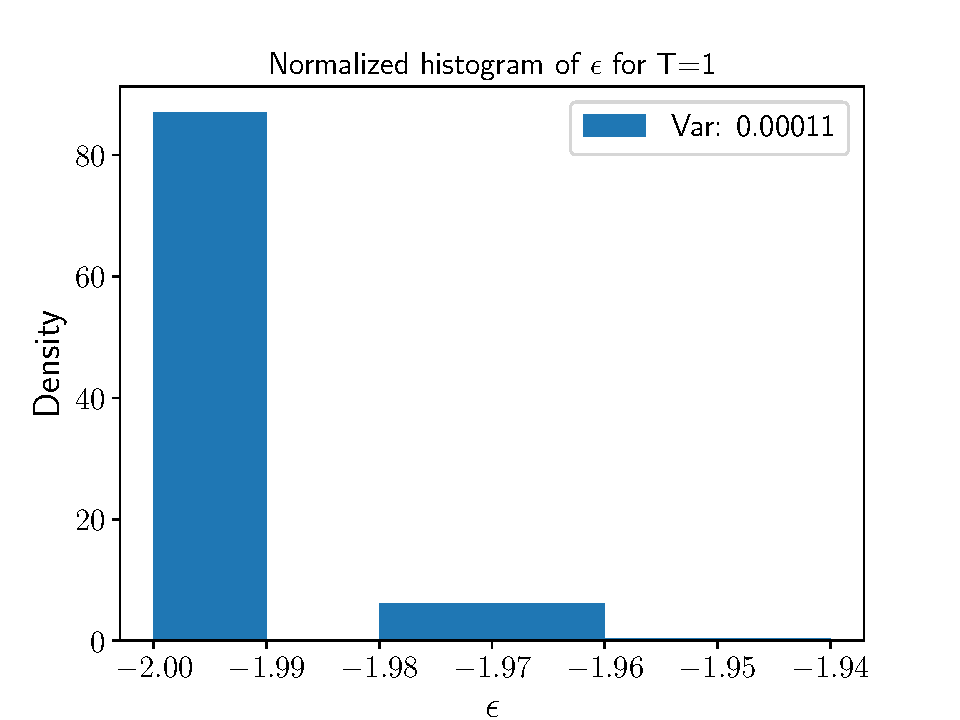
\includegraphics[scale=0.55]{figures/Histo_T1.pdf}
		\caption{}
		\label{fig:hist1}
	\end{figure}

	\begin{figure}[h!]
		\centering
		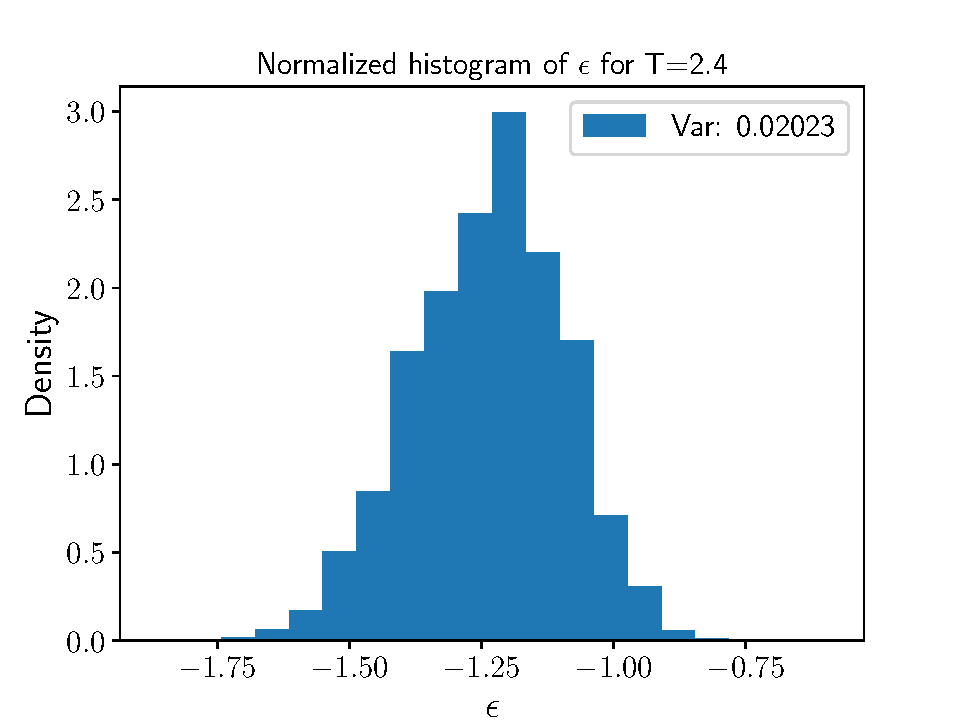
\includegraphics[scale=0.55]{figures/Histo_T2.pdf}
		\caption{}
		\label{fig:hist2}
	\end{figure}

	\subsection{Phase Transition}\label{subsec:num phase transition}

	MOM! IT IS NOT JUST A PHASE!!!!!
	
	% ===========================================
	\section{Discussion}\label{sec:discussion}
	%
	\subsection{Analytical and Numerical for L=2}\label{subsec:dis 2x2}
	
	Figures \ref{fig:chi4} and \ref{fig:cv4} shows the expected value of the susceptibility
	and the heat capacity for different MCMC cycle. We see that we reach quickly the theoretical
	value in 2000 cycles. Increasing the number of cycle will provide better and better 
	approximation as expected. However we notice that we never are perfectly constant and adding
	more cycles does not gives us the assurance that we would reach the theoretical value. This 
	can be explained due to the randomness of our algorithms. Indeed, if we start in a low probability state we can spend some time equilibrating which would weight heavily on the 
	expected value. This two figures shows that the burn in method would improve significantly 
	the numerical value.
	
	
	\subsection{Burn-in}\label{subsec:dis burnin}
	
	We know take a look at the equilibration time. There are many ways of calculating the required
	time for our algorithm to reach equilibrium \colorbox{red}{some citation}. We chose 
	to implement the burn-in method. This method consist in letting our code run for a certain number
	of cycle $N_{\rm burn}$ and once we reach the $N_{\rm burn} + 1$ cycle we consider that we have reached equilibrium and we start saving the data of interest.    
	
	
	\subsection{Distribution of $\epsilon$}\label{subsec:dis epsilon}
	
	\subsection{Parallelization}\label{subsec: dis parallelization}
	
	\subsection{Phase transition and critical temperature}\label{subsec: dis phase transition}
	
	% ===========================================
	\section{Conclusion}\label{sec:conclusion}
	We have studied the 2D Ising model with the Monte Carlo Markov Chain algorithm 
	using the Metropolis algorithm to sample the spin configuration. We found different 
	distribution of $\epsilon$ for different temperature and found out that it plays 
	an important role in the distribution's shape. The main focus on this paper is the 
	phase transition. For different lattice size we iterated over four different lattice 
	size $L=$\{40, 60, 80, 100 \}, used the MCMC algorithm to compute the expected values 
	of $\chi$ and $C_v$. This allowed us to found a critical temperature of $T_c(L=\infty)$
	to be $ 2.29 \pm 0.04 J/k $ where the error is calculated via the fitting function 
	\textit{linregress} from the \textbf{scipy} library. The numerical value is in the range
	of the theoretical value $T_{c}^{\rm th} \approx 2.269 J/k$.
	
	
	\onecolumngrid
	
	%\bibliographystyle{apalike}
	\bibliography{ref}
	
	
\end{document}
